\chapter{Formáty pro efektivní zobrazování velkých snímků na webu}
\label{chap:formats}
V této kapitole bude popsána problematika toho, jak v~rámci webu optimalizovaně zobrazovat snímky s~vysokým rozlišením. Princip je následující, v~případě, že je snímek oddálený, tak uživatel na svém monitoru stejně neuvidí každý detail a~ze serveru se zbytečně stahoval příliš detailní snímek. Přitom by stačilo, kdyby se vždy dostahovala detailněji pouze ta část snímku, na kterou se uživatel zaměří. Přesně tento koncept využívají dlaždicové formáty, jež uchovávají snímky s~různou mírou detailu. Většinou uživatele detailně zajímá pouze část obrázku a~zbytek se stahuje úplně zbytečně. Další výhodou těchto formátů je kromě úspory přenosu dat bezpečnost autorských práv, jelikož snímek nelze tak jednoduše stáhnout. V~případě stažení oddáleného snímku totiž bude výstup v nízké kvalitě. Tyto formáty se často využívají například u webových galerií nebo map, kde není žádoucí provést pouhou kompresi a~poskytnout tak méně kvalitní verzi snímku. Kromě definice samotného formátu k~němu existuje i~podpora knihoven, které s~daným formátem usnadní práci vývojářům.

\section{Deep Zoom Image}
Deep Zoom \cite{MicrosoftDeepZoom} je technologie od společnosti Microsoft určená pro efektivní zobrazování velkých snímků na webu. Technologie nahraje adekvátně kvalitní obrázek vzhledem k~přiblížení a~nabízí podporu jak pro jeden snímek, tak pro celou kolekci snímků. Snímek se při konverzi rozdělí na malé dlaždice a~ty se uspořádají do pyramidového schématu. Při prvotním načtení oddáleného obrázku se použije dlaždice z~vrchu pyramidy, jež na malém rozlišení pokrývá celý snímek v~nízké kvalitě. Jakmile uživatel začne přibližovat snímek, tak se vždy dostahuje detailnější snímek z~nižší vrstvy pyramidy, který na stejném rozlišení vyobrazuje pouze část originálního snímku, takže celkový efekt spočívá v detailnějším snímku pro uživatele, a to bez stahování celého snímku ve velkém rozlišení. 

\begin{figure}[htbp]
\centering
    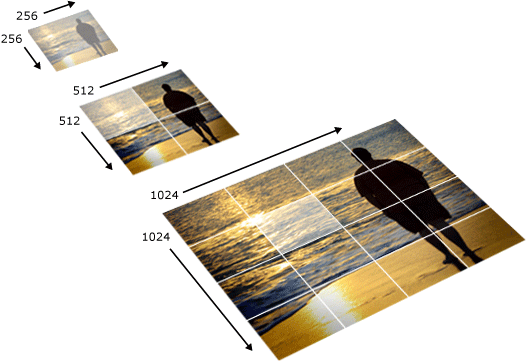
\includegraphics[scale=.5]{obrazky-figures/formats/deepZoom1.png}
    \caption{Rozložení obrázku na dlaždice v~rámci technologie Deep Zoom\protect\footnotemark}
\end{figure}

\newpage
\noindent
Informace o jednotlivých dlaždicích jsou zakódovány následující strukturou \\\texttt{[úroveň]/[sloupec]\_[řádek].[přípona souboru]} ve formátu XML. Na každé úrovni pyramidy je předešlá dlaždice rozložena na čtyři detailnější. Deep Zoom také podporuje řídké obrázky, kde různé části obrázku mohou mít různou úroveň detailu.

\footnotetext{Obrázek pochází ze stejného zdroje jako informace o Deep Zoom formátu.}

\section{Zoomify}
Zoomify \cite{IntroductionZoomifyImage} je konkurenční cross-platform opensource formát k~Deep Zoom image, který vytvořila stejnojmenná společnost. Oba formáty mají mnoho společných rysů a pro popis jednotlivých dlaždic používají formát XML. Snímek je rozkládán do hierarchické pyramidy dlaždic o maximální velikosti $256\times256$ pixelů. V~další vrstvě se dlaždice agregují, takže jedna dlaždice obsahuje data ze čtyř dlaždic nižší úrovně. Dlaždice se tvoří zleva doprava a~následně shora dolů. Indexování obrázků probíhá také obdobně jako u formátu Deep zoom \texttt{[[úroveň]]-[sloupec]\_[řádek].[přípona souboru]}. Indexování začíná od nuly, takže dlaždice, která obsahuje celý obrázek ve velikosti maximálně $256\times256$ pixelů, má souřadnice \texttt{0-0-0.[přípona souboru]}.

\section{International Image Interoperability Framework}
IIIF \cite{IIIFIntroduction} se na rozdíl od předchozích formátů nezaměřuje pouze na snímky, ale řeší poskytování veškerého audiovizuálního obsahu v~rámci webu včetně metadat. Metadata jsou chápána jako data o datech a patří mezi ně například názvy, titulky a~popisy. V~rámci zobrazování snímků podporuje funkci přibližování a~načítání pouze části snímku stejně jako předchozí formáty. Tento aplikační rámec rozděluje svoji funkcionalitu na dvě části, doručování a~zobrazování obsahu. Dále odděluje uložení dat a~metadat, která spojuje na základě definice v~souboru \texttt{manifest.json}. Aplikační rámec IIIF také umožňuje použít stejné standardizované principy, a to například pro poskytování autentizace a~vyhledávání obsahu. 
\newpage
\begin{figure}[htbp]
\centering
    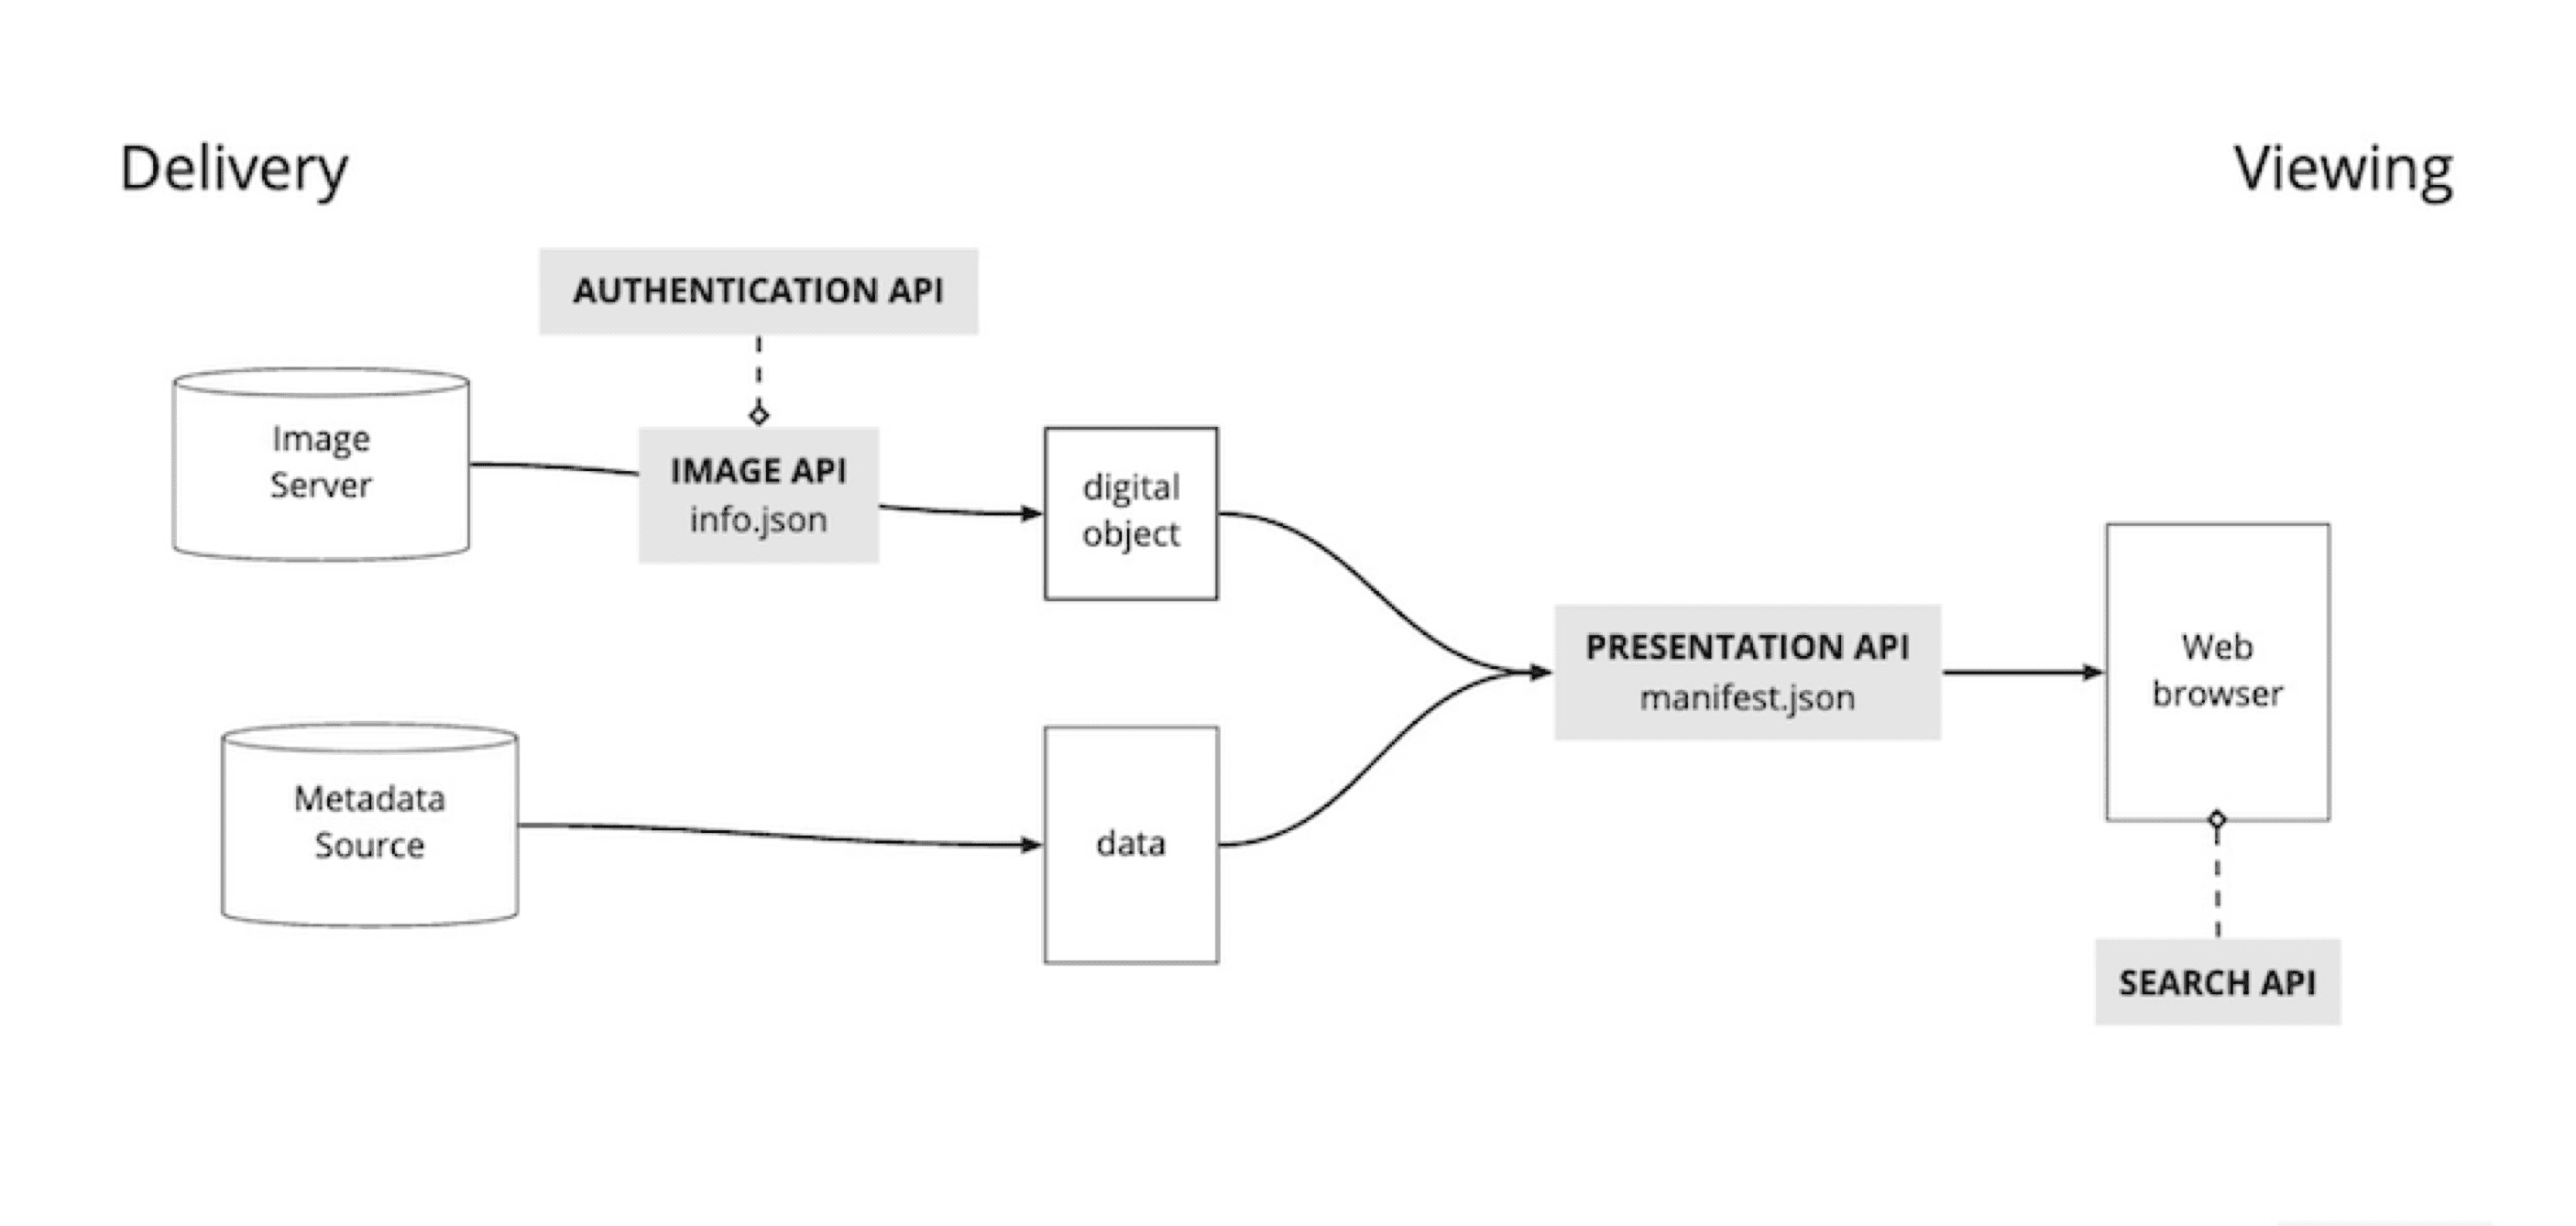
\includegraphics[scale=.15]{obrazky-figures/formats/IIIF_Architecture.png}
    \caption{Architektura pro použití IIIF\protect\footnotemark}
\end{figure}

\noindent
V rámci podpory snímků umožňuje aplikační rámec IIIF do URL volání daného API specifikovat parametry pro volbu výřezu snímku. Dále existují parametry pro nastavení velikostí, rotace a případně filtrů pro výsledný snímek. Oproti ostatním formátům je zde výřez specifikován pozicí levého horního rohu a~následně šířkou a~výškou výřezu, což umožňuje přesně specifikovat část obrázku, která má být zobrazena.

\begin{figure}[htbp]
\centering
    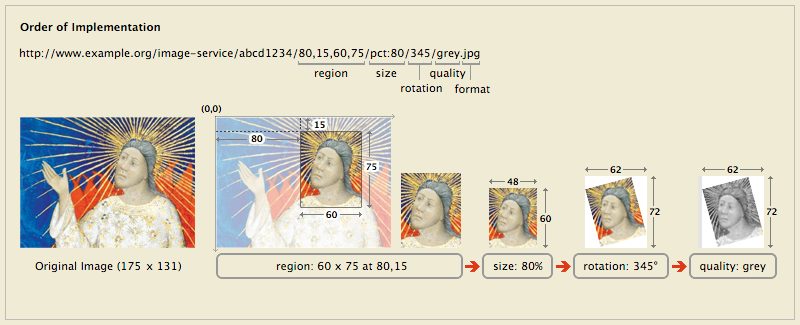
\includegraphics[scale=.45]{obrazky-figures/formats/IIIF_image_processing.png}
    \caption{Zpracování obrázku pomocí IIIF\protect\footnotemark[2]}
\end{figure}
\footnotetext{Obrázek pochází ze stejného zdroje jako informace o IIIF formátu.}